\section{Linear Regression}
\smallskip \hrule height 2pt \smallskip

\underline{Ordinary Least Squares} \hfill \\

Notation:
\begin{itemize}
	\item \textbf{$x_i$}: an input data point.  \_\_ rows by \_\_ columns. 
	\item \textbf{$y_i$}: a predicted output
	\item \textbf{$\widehat{y_i}$}: a predicted output
	\item \textbf{$\widehat{y}$}: 
	\item \textbf{$w_k$}: weight k
	\item \textbf{$\bm{w}*$}:
	\item \textbf{$f_k(x_i)$}
	\item \textbf{$t_j$}: the output variable that you either have data for or are predicting. 
	\item \textbf{$t(\bm{x})$}: Data.  "Mapping from x to t(x)"
	\item \textbf{$H$}: $H = \{ h_1, \dots, h_K \}$.  Basis functions.  In the simplest case, they can just be the value of an input variable/feature or a constant (for bias).  
	\item \textbf{$ || \widehat{w} ||_1$}: "L1" penalty.  The "Manhattan distance".  Like traveling a, b in a pythagorean triangle.  $\sum |x_i|$
	\item \textbf{$ || \widehat{w} ||_2$}.  "L2" penalty.  Euclidean length of a vector.  Like c in a pythagorean triangle.  $\sqrt{\sum |x_i|^2}$	
\end{itemize}

\underline{Vocab}:
\begin{itemize}
	\item \textbf{basis function}
	\item \textbf{bias} - like the intercept in a linear equation.  The part that doesn't depend on the features. 
	\item \textbf{hyperplane} - a plane, usually with more than 2 dimensions. 
	\item \textbf{input variable} - a.k.a. feature.  % https://en.wikipedia.org/wiki/Dependent_and_independent_variables
		E.g. a column like CEO salary for rows of data corresponding to different companies.
	\item \textbf{response variable} - synonyms: "dependent variable", "regressand", "predicted variable", "measured variable", "explained variable", "experimental variable", "responding variable", "outcome variable", and "output variable".   E.g. a predicted stock price.   
	\item \textbf{regularization} -  introducing additional information in order to solve an ill-posed problem or to prevent overfitting. 
	% https://en.wikipedia.org/wiki/Regularization_(mathematics)
	E.g. applying a penalty for large parameters in the model. 
	\item \textbf{ridge regression} - 
	\item \textbf{vector norm}: put in a vector and get out a number like length or size.  Real valued function of some sort of vector or matrix quantity. 
	\item \textbf{hyperparameters}: in Bayesian analysis, the parameters that don't touch the data.  Like the parameters for the prior on the prior.  Called the ridge regression $\lambda$ a hyperparameter, though this is a stretch in the terminology. 
	\item \textbf{feature selection}: explicitly select features that can go into your model instead of throwing all features in. 
	\item \textbf{loss function}: a regularization term, such as squared error $L_2$ for regression
	\item \textbf{training set error}:  *doesn't include the regularization penalty!*.  A.k.a. "training error".  
			Sum of squares error divided by the number of points.   See formula later. 
%	\item \textbf{training error}:  sononomous
\end{itemize}

\underline{Ordinary Least Squares}: \hfill \\
total error = $\displaystyle \sum_i (y_i-\hat{y_i})^2 = \sum_i(y_i - \sum_k w_k f_k(x_i))^2$ \hfill \\
Under the additional assumption that the errors be normally distributed, OLS is the maximum likelihood estimator. \hfill \\ % https://en.wikipedia.org/wiki/Ordinary_least_squares
?? Use words to describe what subset of regression in general this is.  What is ordinary? What are we limiting?  \hfill \\
 \hfill \\

The regression problem: \hfill \\
Given basis functions $\{ h_1, \dots, h_K \}$  with $h_i(\bf{x}) \in \mathbb{R}$,  \hfill \\
	find coefficients $\bm{w} = \{ w_1, \dots, w_k \}$.  \hfill \\%  
$t(\bm{x}) \approx \widehat{f}(\bm{x}) = \sum_i w_i h_i(\bm{x})$ 

This is called linear regression b/c it is linear in the parameters. 
We can still fit to nonlinear functions by using nonlinear basis functions. 
Minimize the \textbf{residual squared error}: \hfill \\
$ \displaystyle \bm{w}* = \argmin_{\bm{w}}  \sum_j (t(\bm{x}_j) - \sum_i w_i h_i(\bm{x}_j))^2$
\hfill \\  \hfill \\

For fitting a line in 2D space, your basis functions are $\{ h_1(x) = x, h_2(x) = 1 \}$  \hfill \\  \hfill \\

To fit a parabola, your basis functions could be $\{ h_1(x) = x^2, h_2(x)=x, h_3(x)=1 \}$.   \hfill \\
Want a 2D parabola? Use $\{ h_1(x) = x_1^2, h_2(x)=x_2^2, h_3(x)=x_1 x_2, \dots \}$. \hfill \\
Can define any basis functions $h_i(\bm{x})$ for n-dimensional input $\bm{x} = <x_1, \dots, x_n>$
\hfill \\  \hfill \\

\underline{Regression: matrix notation}: \hfill \\
\begin{align*}
	\bm{w}* &= \argmin_w \sum_j(t(\bm{x}_j - \sum_i w_i h_i(\bm{x}_j))^2  \\
	\bm{w}* &= \argmin_w (\bm{Hw} -\bm{t})^T (\bm{Hw} -\bm{t})
\end{align*}
$  (\bm{Hw} -\bm{t})^T (\bm{Hw} -\bm{t})$ is the residual error. 
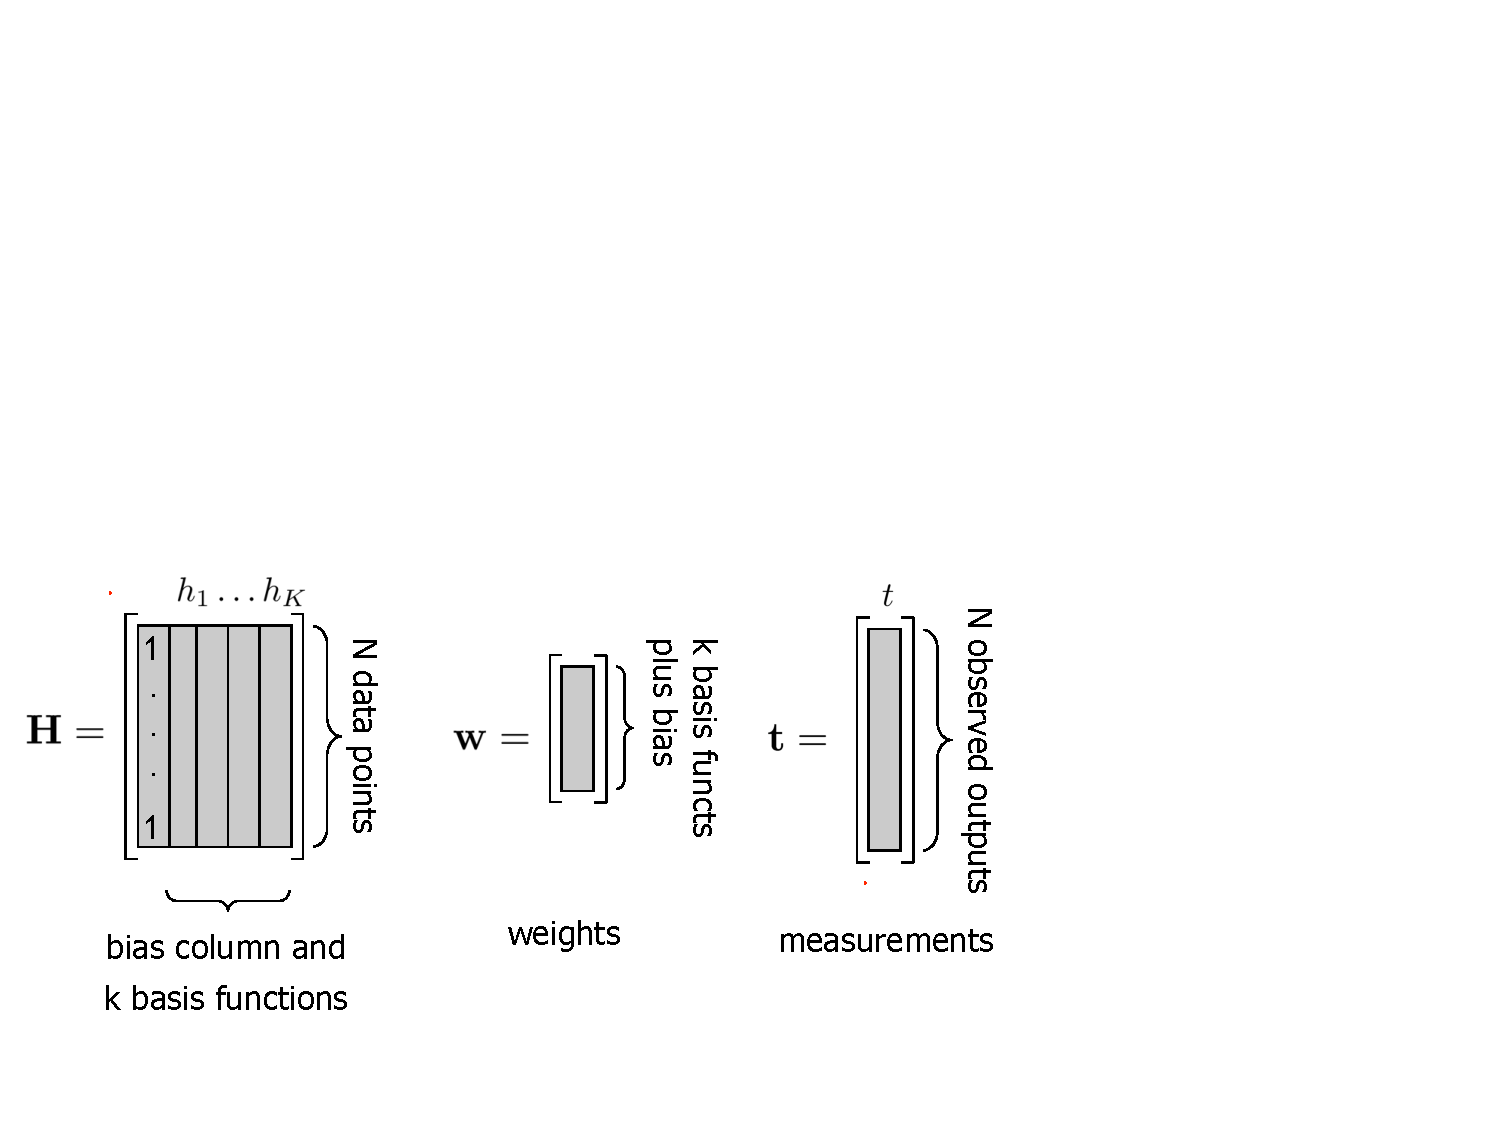
\includegraphics[width=3in]{figures/Least_squares_matricies.pdf}

\underline{Regression: closed form solution}:  % derivation: http://courses.cs.washington.edu/courses/cse446/16wi/Slides/4_LinearRegression.pdf
\begin{align*}
	\bm{w}^* = \argmin_w (\bm{Hw} -\bm{t})^T (\bm{Hw} -\bm{t})  & \\
	\bm{F}(\bm{w}) =  \argmin_w (\bm{Hw} -\bm{t})^T (\bm{Hw} -\bm{t}) & \\
	\triangledown_{\bm{w}}\bm{F}(\bm{w}) = 0 \\
	2 \bm{H}^T (\bm{H}\bm{w}-\bm{t}) = 0  & \\
	(\bm{H}^T\bm{H}\bm{w}) - \bm{H}^T\bm{t} = 0 & \\
	\bm{w}^* = (\bm{H}^T\bm{H})^{-1}\bm{H}^T\bm{t} &
\end{align*}

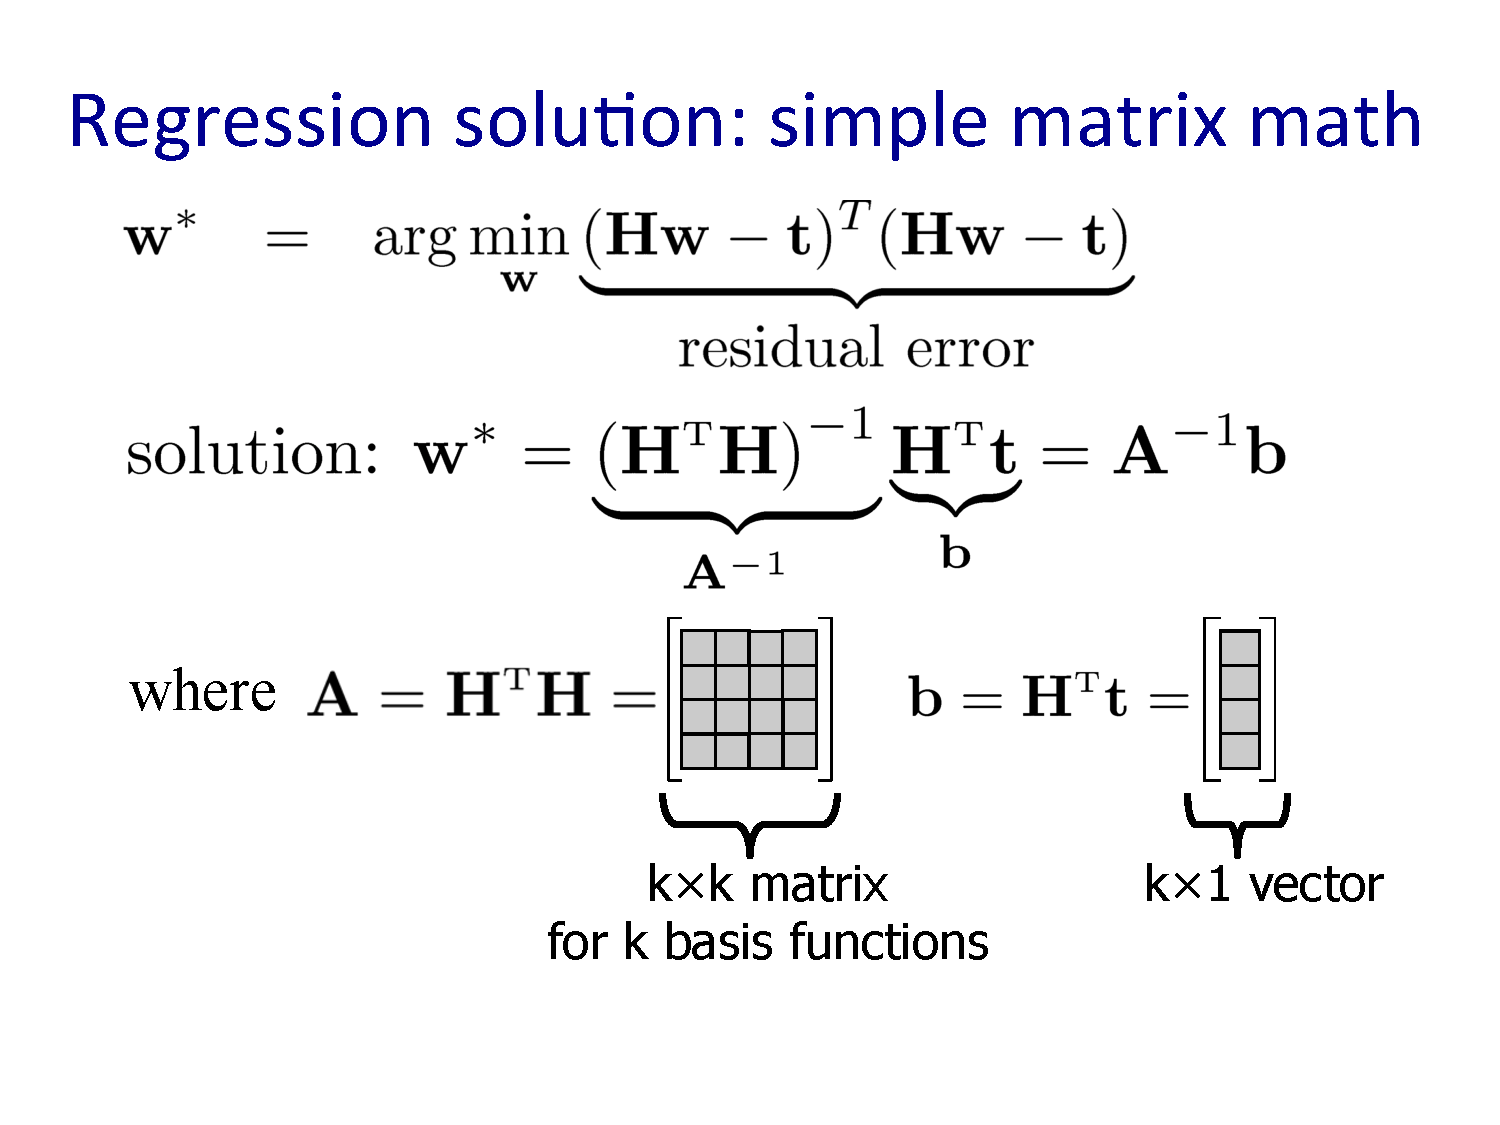
\includegraphics[width=3in]{figures/Regression_matrix_math.pdf}

Linear regression prediction is a linear function plus Gaussian noise:  \hfill \\
$t(\bm{x}) = \sum_i w_i h_i(\bm{x}) + \epsilon $ \hfill \\
We can learn $\bf{w}$ using MLE: 
$P(t | x, w, \sigma) = \frac{1}{\sigma \sqrt{2 \pi}} e^\frac{-[t - \sum_i w_i h_i(x)]^2}{2 \sigma^2}$
Take the log and maximize with respect to w:  (maximizing log-likelihood with respect to w) \hfill \\
$\displaystyle \ln P(D | \bm{w}, \sigma) = \ln(\frac{1}{\sigma \sqrt{2 \pi}})^N \prod_{j=1}^N e^\frac{-[t_j - \sum_i w_i h_i(x_j)]^2}{2 \sigma^2}$ \hfill \\
Now find the w that maximizes this: \hfill \\
$\argmax_w \ln(\frac{1}{\sigma \sqrt{2 \pi}})^N + \sum_{j=1}^N \frac{-[t_j - \sum_i w_i h_i(x_j)]^2}{2 \sigma^2}$ \hfill \\
the first term isn't impacted by $w$ so  \hfill \\
$= \argmax_w  \sum_{j=1}^N \frac{-[t_j - \sum_i w_i h_i(x_j)]^2}{2 \sigma^2}$ \hfill \\
switch to $\argmin_w$ when we divide by -1.  The numerator is constant.:  \hfill \\
$= \argmin_w  [t_j - \sum_i w_i h_i(x_j)]^2 $ \hfill \\

\textbf{Least-squares Linear Regression is MLE for Gaussians!!!}  \hfill \\ \hfill \\

\subsection{Regularization in Linear Regression}  \hfill \\

\subsubsection{Ridge Regression}  \hfill \\
Here is our old "ordinary" least squares objective function:   \hfill \\
$\displaystyle \widehat{w} = \argmin_w \sum_{j=1}^N [t(x_j) - (w_0 + \sum_{i=1}^k w_i h_i(x_j))]^2$   \hfill \\
It is the same as the previous ones but $i=0$ is pulled out.    \hfill \\
Now for ridge regression, we use that same notation.  \hfill \\
And we add a penalty term that isn't applied to the bias feature:
\begin{align*}
	\widehat{w}_{ridge} &= \argmin_w \sum_{j=1}^N [t(x_j) - (w_0 + \sum_{i=1}^k w_i h_i(x_j))]^2 + \lambda \sum_{i=1}^k w_i^2   \\
	&= \argmin_w (\bm{H}\bm{w} - \bm{t})^T(\bm{H}\bm{w}-\bm{t}) + \lambda \bm{w}^T I_{0+k} \bm{w}
\end{align*}
That $I_{0+k}$ matrix is this: 
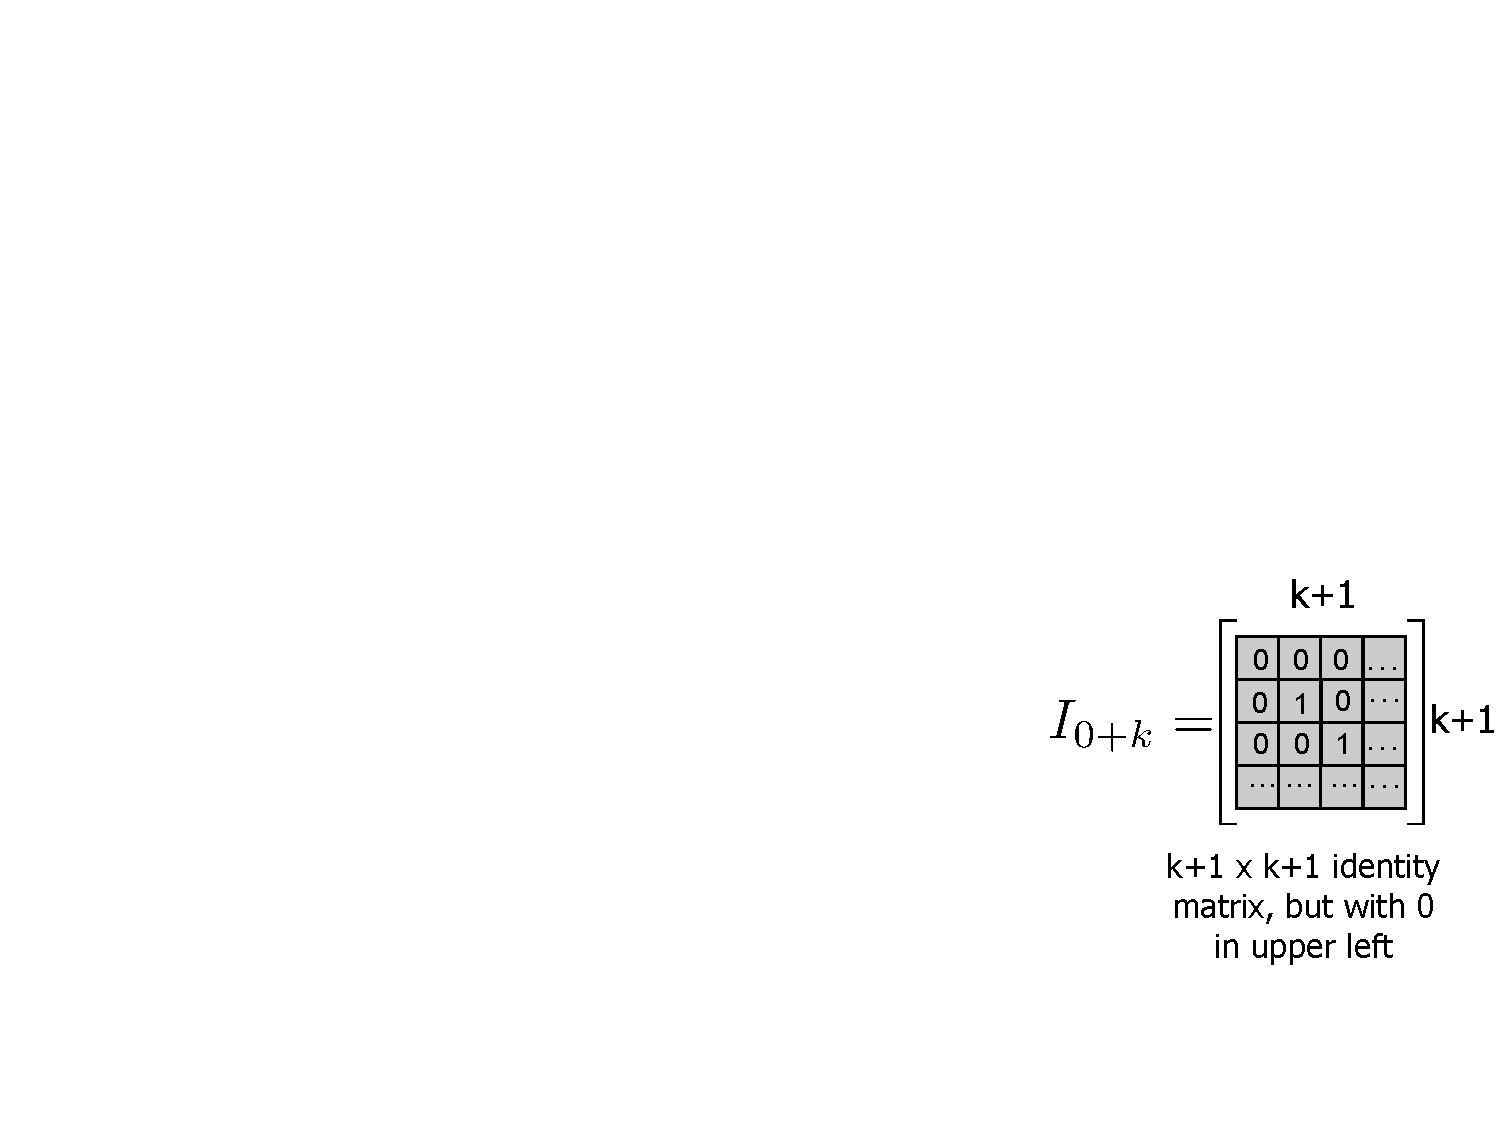
\includegraphics[width=1.0in]{figures/ridge_identity_matrix_with_zero.pdf}  \hfill \\
% Erick hasn't seen this notation.
Allows you to multiply the whole weight array without getting the bias term in there. 

A similar derivation leads to a closed form solution:  \hfill \\
% http://courses.cs.washington.edu/courses/cse446/16wi/Slides/4_LinearRegression.pdf 
$w_{ridge}^* = (\bm{H}^T\bm{H} + \lambda I_{0+k})^{-1}\bm{H}^T\bm{t}$ \hfill \\
(Recall that un-regularized regression was $w^* = (\bm{H}^T\bm{H})^{-1}\bm{H}^T\bm{t}$).  \hfill \\   \hfill \\

How do you chose how large $\lambda$ is? \hfill \\
* As $\lambda \rightarrow 0$, becomes same as MLE: unregularized.  Large magnitudes of coefficients. \hfill \\
* As $\lambda \rightarrow \infty$, all weights become 0.  \hfill \\   \hfill \\

\underline{Experiment cycle}: 
\begin{enumerate}
	\item select a hypothesis $f$ to best match the training set. 
	\item isolate a held-out data set if you have enough data, or do K-fold cross-validation if not enough data. 
	\begin{itemize}
		\item tune hyperparameters ($\lambda$) on the held-out set or via crossvalidation.  (Try many values of $\lambda$ and chose the best one.)  
		\item If doing K-fold, divide the data into k subsets.  
				Repeatedly train on k-1 and test on the remaining one.  
				Average the results. 
	\end{itemize}
\end{enumerate}

\underline{Regularization options}: Ridge vs Lasso.  \hfill \\
Ridge: 
\begin{itemize}
	\item $ \displaystyle \widehat{w}_{ridge} = \argmin_w \sum_{j=1}^N [t(x_j) - (w_0 + \sum_{i=1}^k w_i h_i(x_j))]^2 + \lambda \sum_{i=1}^k w_i^2   $ 
	\item L2 penalty   
\end{itemize}
Lasso: \hfill \\
\begin{itemize}
	\item$ \displaystyle \widehat{w}_{ridge} = \argmin_w \sum_{j=1}^N [t(x_j) - (w_0 + \sum_{i=1}^k w_i h_i(x_j))]^2 + \lambda \sum_{i=1}^k |w_i|   $ 
	\item L1 penalty: linear penalty pushes more weights to zero.  Allows for a type of feature selection.  But it is not differentiable and there is no closed form solution. 
\end{itemize}

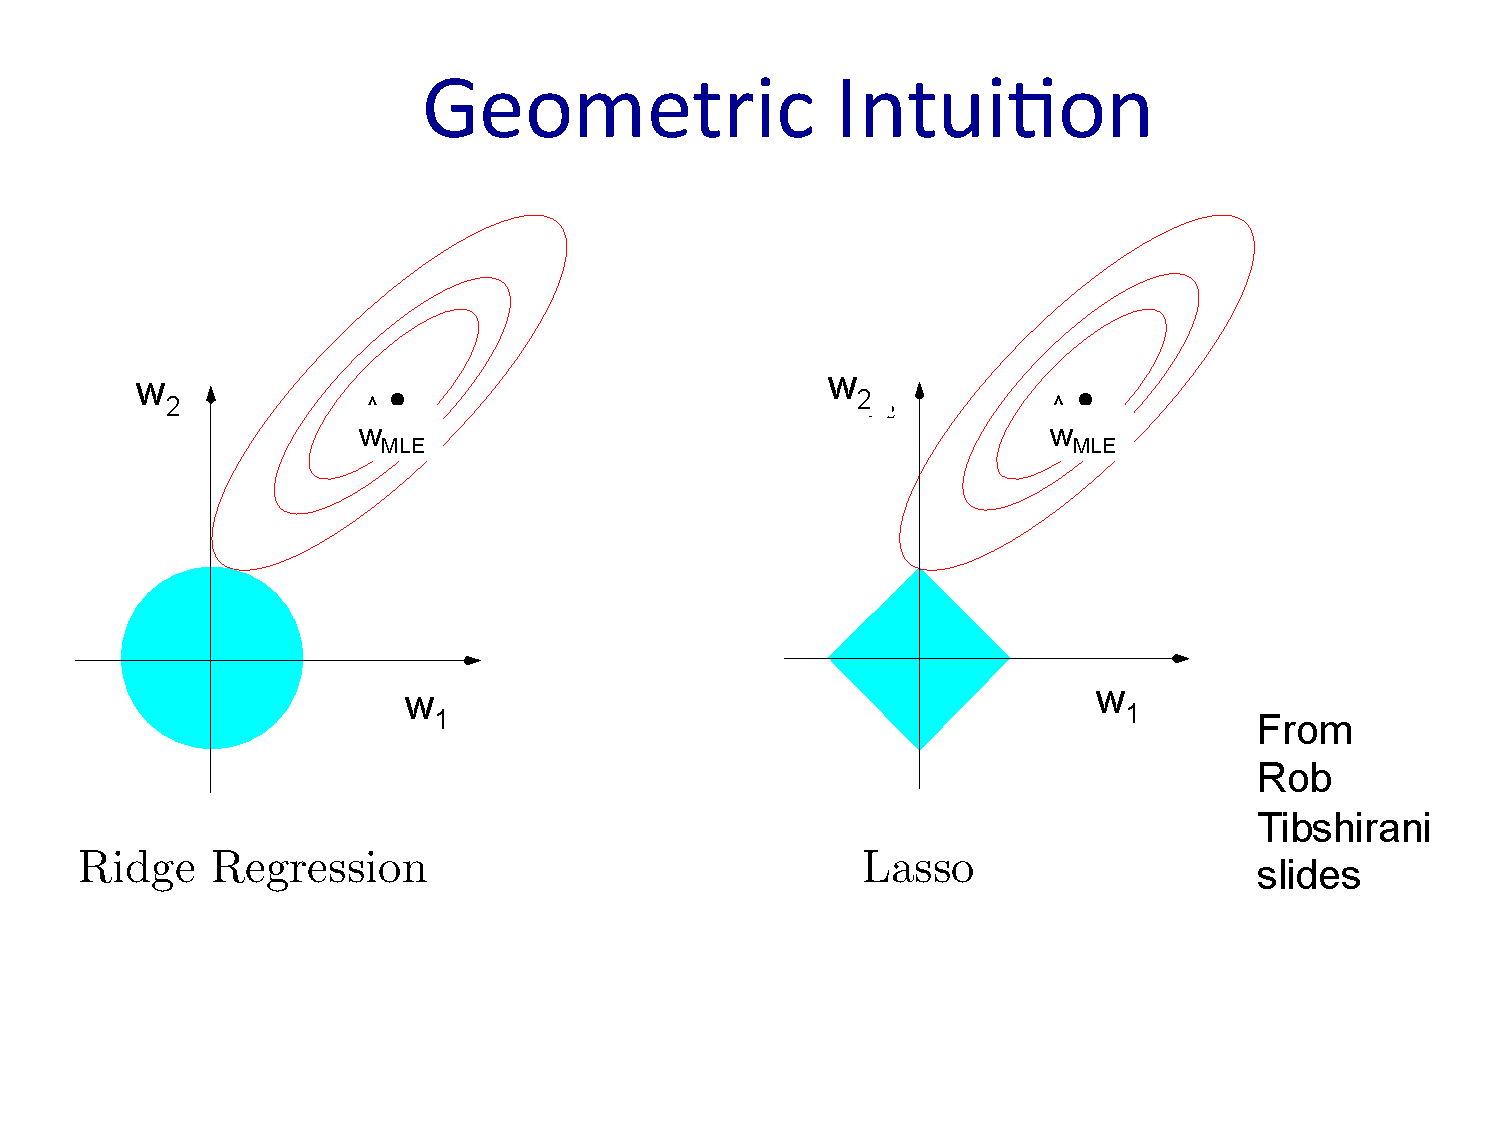
\includegraphics[width=3in]{figures/lasso_and_ridge_geometry.pdf}

This figure shows: 
\begin{itemize}
	\item The contour lines represent the maximum likelihood of the vector of weights.  
		All points on the contour have equal likelihood.
	\item The two axes represent different parameters for two of the weights.  (regression coefficients)
	\item Circles are characteristic of ridge regression (with L2 penalty): Penalty = the magnitude of the vector.
	\item Shapes that are pointy on the axes are characteristic of Lasso (with L1 penalty): the vector components get added. 
	\item Where the likelihood function touches in this $w_1, w_2$ space represents the coefficients of the weights.
		For Ridge Regression, we see that small but nonzero values of the coefficients can be obtained.
		For Lasso Regression, the curves are most likely to touch the diamond on the axes, 
		resulting in coefficients that are truly zero. 
\end{itemize} 

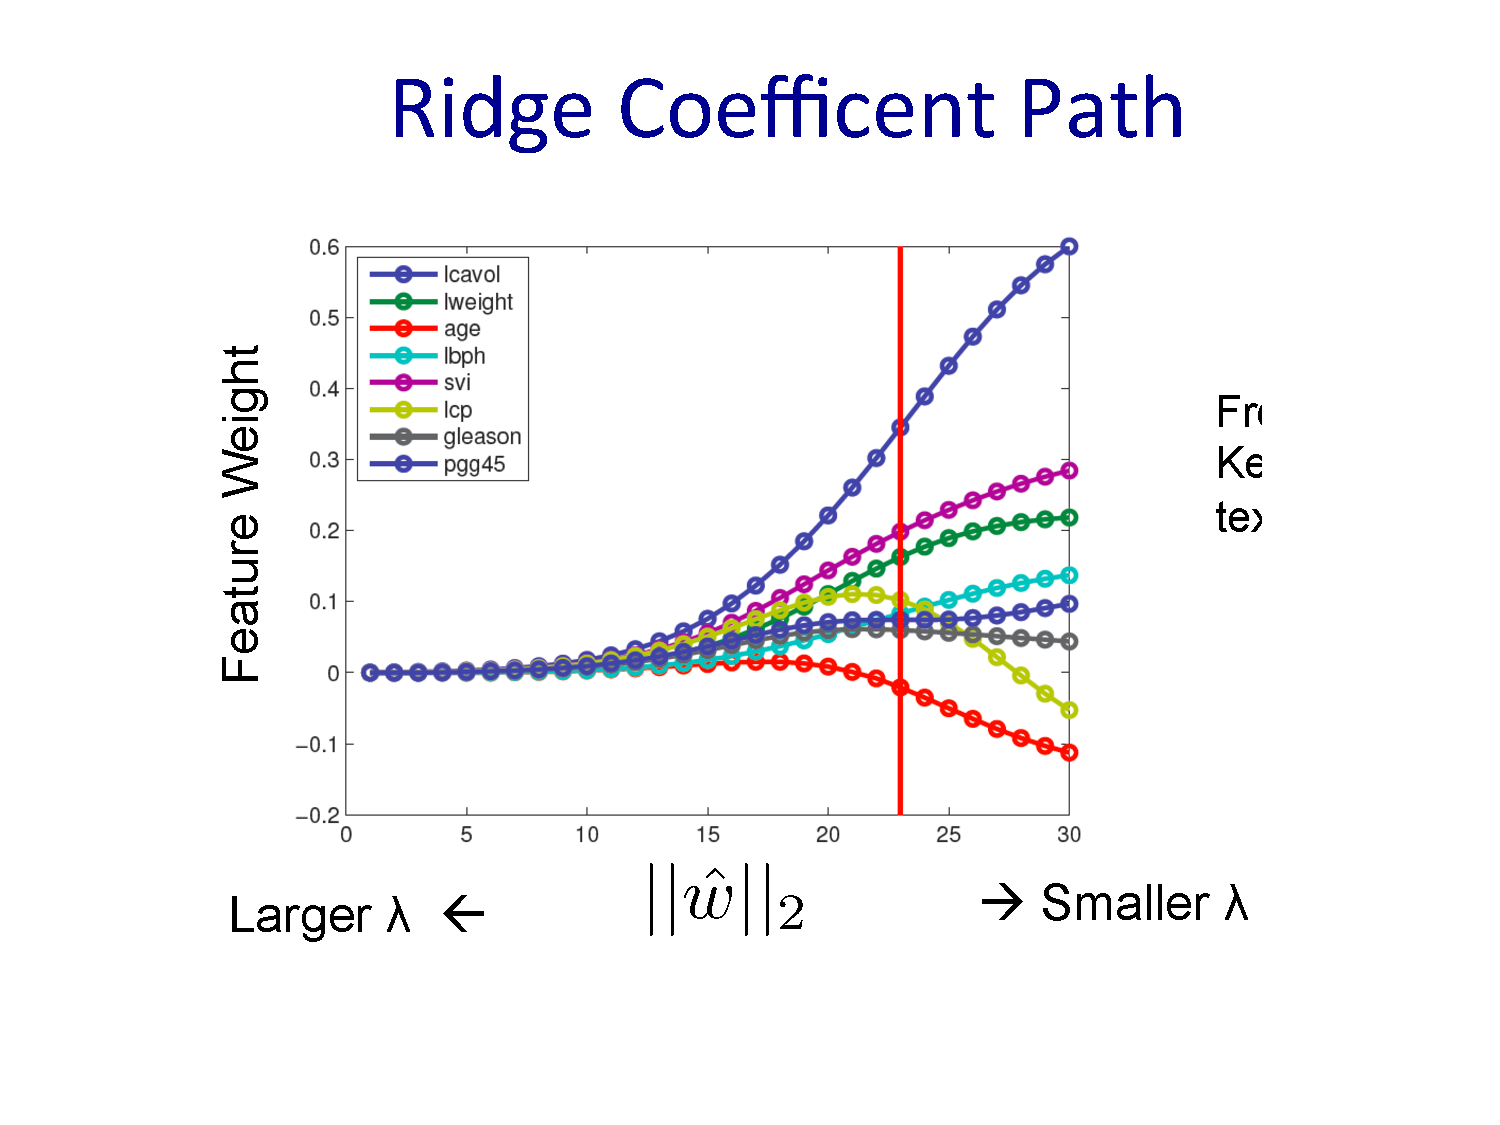
\includegraphics[width=1.8in]{figures/lambda_with_w2.pdf}  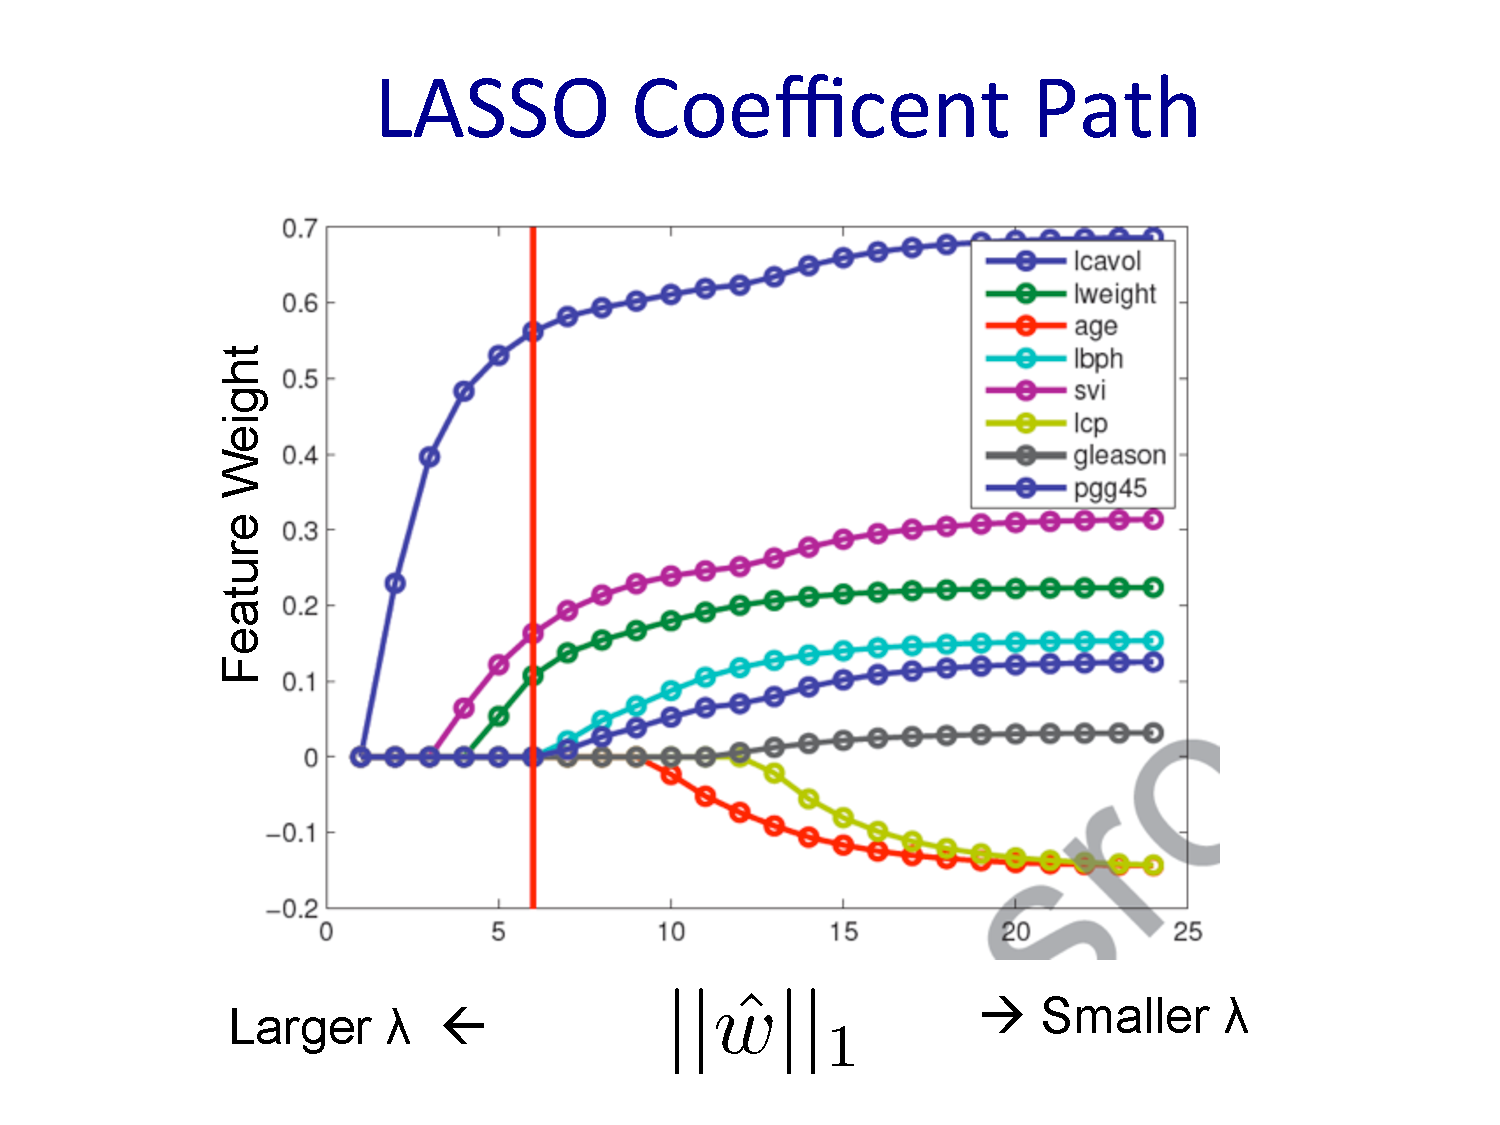
\includegraphics[width=1.6in]{figures/lambda_with_w1.pdf}
Don't compare coefficient magnitudes at given $\lambda$s, 
but do note that for Ridge the gradually come away from the zero axis and in Lasso they are zero until they pop out.   \hfill \\ \hfill \\

\underline{Bias-Variance Tradeoff}:   \hfill \\
Your choice of hypothesis class (e.g. degree of polynomial) inroduces learning bias.  \hfill \\
\textbf{A more complex class } $\rightarrow$ less bias and more variance.  \hfill \\  \hfill \\

\underline{Training Set Error}:  (training error) \hfill \\
$\displaystyle  error_{train}(\bm{w}) = \frac{1}{N_{train}} \sum_{j=1}^{N_{train}}(t(\bm{x_j})-\sum_{i} w_i h_i(\bm{x_j}))^2$
Decreases exponentially with model complexity.  
\hfill \\  \hfill \\
% http://courses.cs.washington.edu/courses/cse446/16wi/Slides/4_LinearRegression.pdf

\underline{Prediction Error}:   \hfill \\
Since the training set error can be a poor measure of the "quality" of the solution, we can use prediction error ("true error").  
The error over all possibilities.   Instead of sum, take expectation. 
\begin{align*}
	error_{true}(\bm{w}) &= E_X[(t(\bm{x_j})-\sum_{i} w_i h_i(\bm{x_j}))^2] \\
					&= \int_x (t(\bm{x_j})-\sum_{i} w_i h_i(\bm{x_j}))^2 p(\bm{x}) d\bm{x}
\end{align*}
How to get $p(\bm{x})$?  Need to know the true distribution of the data (?) \hfill \\
Prediction error is high when the model is too simple \underline{and} too complex, unlike training set error which only penalizes too simple. 

